%
% path-finding
% @author Tobias Weber <tweber@ill.fr>
% @date 2021
% @license see 'LICENSE' file
%

This chapter is devoted to the development of the theoretical frameworks for path-finding in a triple-axis spectrometer (TAS). 
The path should furthermore be optimal in the sense that the instrument not only avoids obstacles like walls or equipment in 
the experimental area, but also keeps a maximum distance from them.

Before looking at the situation with TAS in section \ref{sec:tasrobot}, we shortly review the ideas of motion planning for a 
point-like robot in section \ref{sec:pointrobot}.



\section{Motion planning for a point-like robot}
\label{sec:pointrobot}

\subsection*{Sector-based method}
An algorithm for motion planning in a point-like robot based on decomposing the available space into sectors is 
given in Ref. \cite[Ch. 13, pp. 283-306]{Berg2008}, whose descriptions we follow in this section. 
While the book chapter also describes polygonal robots, we limit ourselves to the parts of the chapter 
that are relevant for the present work.

The movement of the point-like robot in question is not restricted to conventional Cartesian space, its coordinates are given in configuration
space  \cite[Ch. 13.1, pp. 284-286]{Berg2008}, which comprises its inherent degrees of freedom and can -- for instance -- include angular motion.

The algorithm consists of two parts: First, the separation of allowed space into sectors, within which the robot can move 
without hitting an obstacle \cite[p. 286]{Berg2008}. 
The second part concerns the computation of the actual path and is given in Ref. \cite[p. 289]{Berg2008}. 
In the first part, a trapezoidal map (explained below) is created for the configuration space containing the obstacles, 
both of polygonal shape. The trapezoids inside the obstacles are removed form the final map as the robot has to stay clear 
of them. The second part of the algorithm calculates the path of the robot by finding the trapezoids which contain the start 
and goal points, and finding the edges between adjacent trapezoids from starting to ending trapezoid via a breadth-first search in the 
trapezoidal map. The robot will thus first move to the centre of its containing trapezoid, followed by the centre of an edge connecting 
the current to the next trapezoid, next to the centre of the next trapezoid, and so forth until it arrives at its goal. 
The situation is depicted in Fig. \ref{fig:robot_trapezoids}, where we restrict ourselves to line-like obstacles for simplicity, effectively
only using the second part of the algorithm.

Trapezoidal maps and the algorithm for their calculation are given in Ref. \cite[Ch. 6, pp. 121-146]{Berg2008}. Basically, the map of
trapezoids is obtained by extending vertical lines from every vertex in a collection of line segments. The vertical
extensions reach out until they intersect with another line segment of the collection, or an outer bounding box. The original line 
segment and the intersected segment on top (or bottom, respectively) together with the vertical lines form a trapezoid, as shown in 
Fig. \ref{fig:robot_trapezoids}. Together with the trapezoid map, the algorithm constructs in $O \left(n \log_{2} n \right)$ time a data 
structure, which allows querying for the trapezoid containing a given point with time complexity $O \left( \log_{2} n \right)$, 
where $n$ is the number of line segments \cite[Theorem 6.3, p. 133]{Berg2008}.

\begin{figure*}[htb]
	\centering
	\includegraphics[width = 0.4 \textwidth]{figures/pointrobot_walls.pdf}
	\hspace{1 cm}
	\includegraphics[width = 0.4 \textwidth]{figures/pointrobot_walls_trapezoids.pdf}
	\caption{Left panel: A point-like robot has to find a way around line segments which represent obstacles. Right panel: 
		The algorithm outlined in Ref. \cite[p. 289]{Berg2008} constructs a trapezoid map and moves the robot on the
		shortest path from the centre of one trapezoid to the centre of the edge connecting to the next trapezoid, to the
		centre of that trapezoid, and so forth (blue arrows).}
	\label{fig:robot_trapezoids}
\end{figure*}

While the present algorithm can be extended towards polygonal robots \cite[Ch. 13.3, pp. 290-297]{Berg2008} and provides
some useful ideas, it has several severe drawbacks. First and foremost, the trapezoid map cannot handle the case when
two or more line segment vertices coincide, making it very difficult to model polygonal obstacles and not only using mere
line segments. Second, our own implementation has shown that for the algorithm to be stable, it has to handle many 
special cases, for example to eliminate vertices with equal $x$ coordinate components or vertical lines.

\vspace{0.5cm}

\subsection*{Retraction method}
Apart from decomposing the available configuration space into sectors, a more direct approach can be taken. This
approach is called the retraction method and is based on constructing the Voronoi regions of the obstacles and moving
the robot along the Voronoi edges, which ensures that the path is optimal in the sense that the robot is always at
the farthest distance from any obstacle \cite[pp. 163 and 304]{Berg2008}. An example path for the same problem as before
is given in Fig. \ref{fig:robot_voronoi}. It is this approach we will follow for TAS motion planning.

\begin{figure}[htb]
	\centering
	\includegraphics[width = 0.4 \textwidth]{figures/pointrobot_walls_voronoi.pdf}
	\caption{The accessible configuration space is subdivided into the Voronoi regions of the obstacles (coloured). The optimal
		path (blue arrows) in the sense that it keeps the robot at maximum distance from any obstacle, has it move along the 
		Voronoi edges.}
	\label{fig:robot_voronoi}
\end{figure}



\section{Motion planning for a triple-axis spectrometer}
\label{sec:tasrobot}

As it is imperative that the instrument not move into any walls, we choose the retraction method using the obstacles' Voronoi regions.
As for a TAS several coordinate systems are available, we have several equivalent possibilities to describe its movement. 

\subsection*{Instrument positions configuration space}
The first possibility would be to model the entire instrument as a polygonal robot arm and directly use the position of the robot as
its configuration space. This way it would be directly possible to use a polygonal representation of the walls and construct their
Voronoi regions -- or even trapezoidal maps -- as discussed in Sec. \ref{sec:pointrobot}. The main problem with this approach is the
very complicated treatment necessary for the instrument itself.

\subsection*{Crystal coordinates configuration space}
A better way is to use a configuration space where the instrument is represented as a single point in that space. This comes at the 
cost of the shape of the walls becoming more complicated when transformed into configuration space, 
they may not even be simply-connected anymore in that space. There
are two choices for such a configuration space: We can either use the reciprocal crystal coordinates as discussed in Ch. \ref{ch:xtal}
or use a configuration space comprised of the instrumental angles.

Using the reciprocal crystal coordinates as configuration space would need a transformation of the walls into the four-dimensional reciprocal space (three momentum and on energy coordinate). Even when taking into account that the TAS is usually restricted
to a two-dimensional scattering plane, thereby dropping one of the momentum dimensions, the problem would still be 
three-dimensional.

\subsection*{Instrument angles configuration space}
On the other hand, using the instrument angles seems to be even more complicated at first glance. The instrument comprises
six angles, namely the crystal and scattering angles for the monochromator, the sample and the analyser crystals, respectively,
leading to a six-dimensional configuration space. When can take into account that not all angles are independent of one another:
The monochromator and analyser scattering angles are always double their respective crystal angles, because they both
have to fulfill the Bragg condition. We are therefore left with four independent angles: the monochromator and analyser 
scattering angles as well as the sample crystal and scattering angle. 

We are mainly interested in collisions of the instrument with walls or itself, this way the sample crystal angle can be dropped 
from the analysis, because it only rotates the sample axis, but does not move the instrument. It can still lead to forbidden 
positions if it rotates too far and rips out cables or tubes, but these cases we can treat as their own one-dimensional problem. 

A further simplification is possible when taking into account that during a typical experiment the instrument usually only moves 
either its monochromator or analyser angle to choose the energy transfer, but not both. Therefore, one of these angles, 
usually the analyser angle, rests at a constant value. In total, we are left with a two-dimensional configuration space comprised 
of the monochromator and the sample scattering angle. A typical situation is shown in Fig. \ref{fig:tas_wall}. Here, the instrument 
motion is blocked by an obstacle in the experimental zone. The configuration space image shows that the obstacle transforms
into a non-primitive geometric object in configuration space, which -- as already mentioned -- does not even have to be simply-connected.

\begin{figure}[htb]
	\centering
	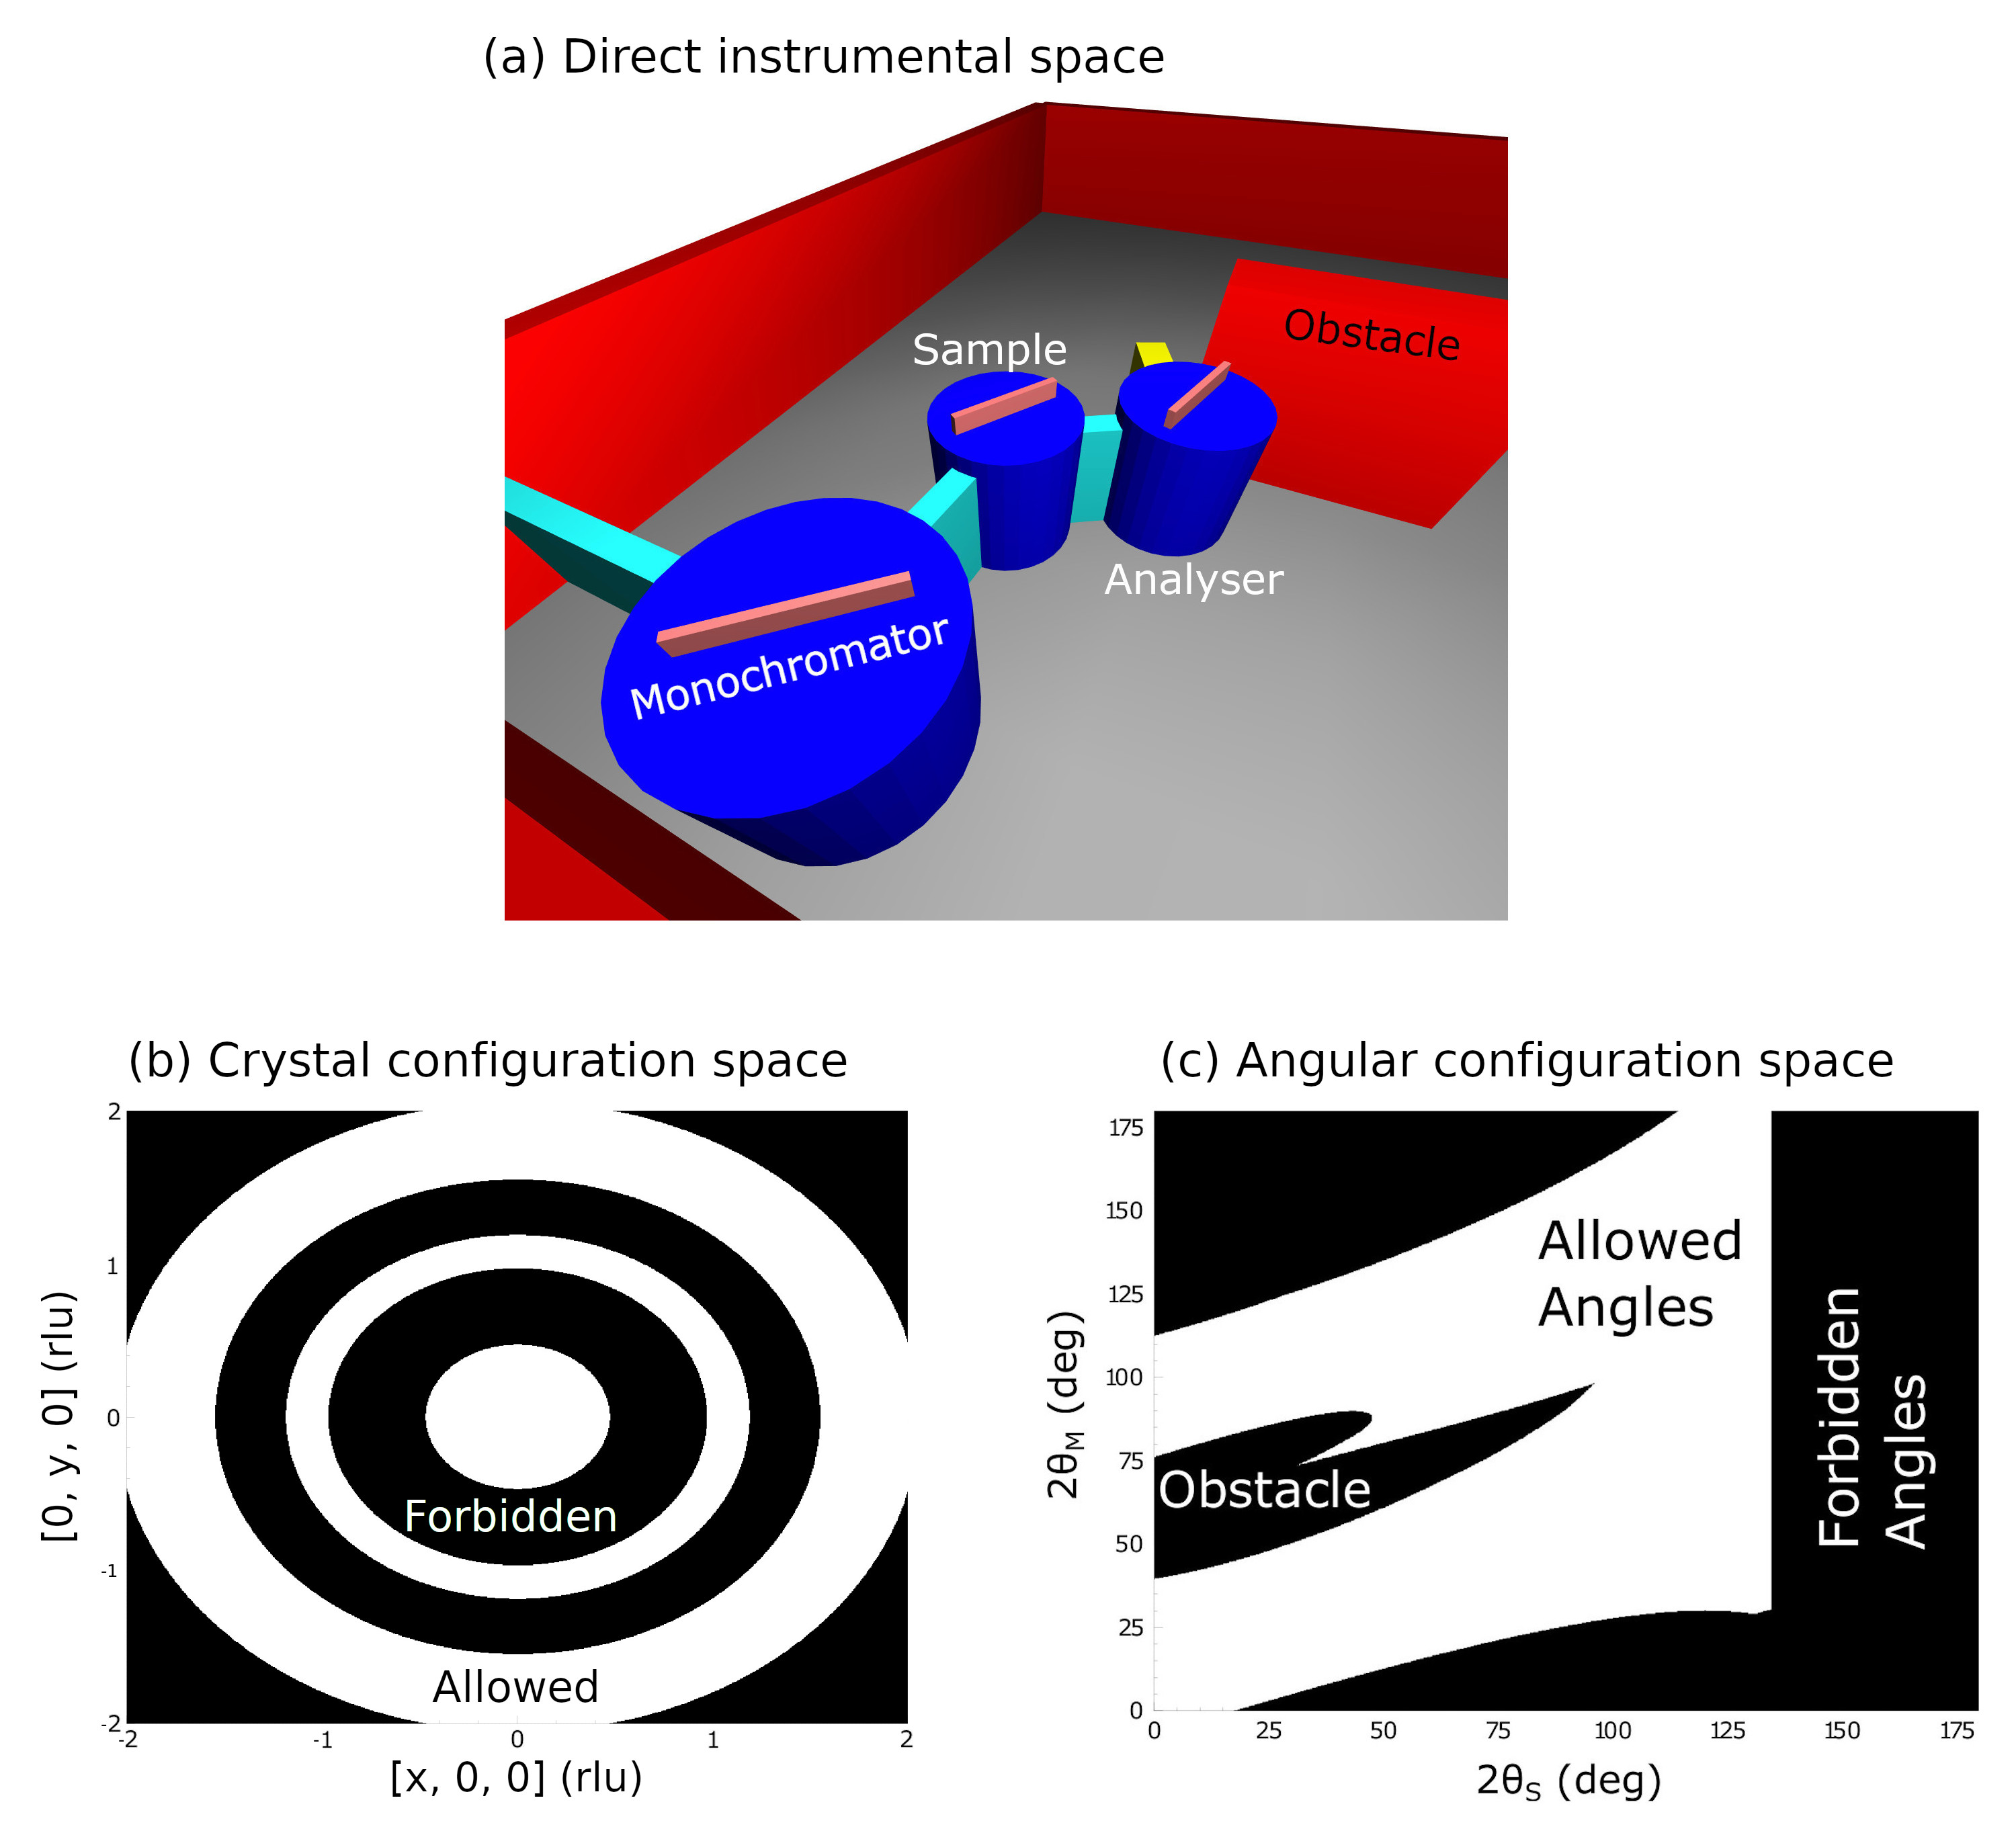
\includegraphics[width = 0.95 \textwidth]{figures/tas_wall.jpg}
	\caption{An obstacle in the instrument space (left) and in the angular configuration space (right). In the configuration
		space, allowed instrument angular positions are shown in white, forbidden positions in black. The outer areas
		of disallowed positions are given either by collisions of the instrument with the outer walls or with itself.}
	\label{fig:tas_wall}
\end{figure}


\section{Finding the Voronoi regions}
TODO
